\documentclass{article}
% if you need to pass options to natbib, use, e.g.:
%     \PassOptionsToPackage{numbers, compress}{natbib}
% before loading neurips_2020
% ready for submission
% \usepackage{neurips_2020}
% to compile a preprint version, e.g., for submission to arXiv, add add the
% [preprint] option:
%     \usepackage[preprint]{neurips_2020}
% to compile a camera-ready version, add the [final] option, e.g.:
     \usepackage[final]{neurips_2020}
% to avoid loading the natbib package, add option nonatbib:
%     \usepackage[nonatbib]{neurips_2020}
\usepackage[utf8]{inputenc} % allow utf-8 input
\usepackage[T1]{fontenc}    % use 8-bit T1 fonts
%\usepackage{hyperref}       % hyperlinks
\usepackage{url}            % simple URL typesetting
\usepackage{booktabs}       % professional-quality tables
\usepackage{amsfonts}       % blackboard math symbols
\usepackage{nicefrac}       % compact symbols for 1/2, etc.
\usepackage{microtype}      % microtypography
\usepackage{tikz}
\usepackage{amssymb}
\usepackage{amsthm}
\usepackage{amsmath}
\usepackage{mathabx}
\usepackage{natbib}
\usepackage{listings}
\usepackage{bbm}
\usepackage{caption}
\usepackage{float}
\usepackage{setspace}
\usetikzlibrary{patterns}
\title{Incentive Incompatibility of Logistic Regression}
% The \author macro works with any number of authors. There are two commands
% used to separate the names and addresses of multiple authors: \And and \AND.
%
% Using \And between authors leaves it to LaTeX to determine where to break the
% lines. Using \AND forces a line break at that point. So, if LaTeX puts 3 of 4
% authors names on the first line, and the last on the second line, try using
% \AND instead of \And before the third author name.
\author{}
\begin{document}
\newtheorem{thm}{Theorem}
\newtheorem{cor}{Corollary}
\newtheorem{lem}{Lemma}
\newtheorem{prop}{Proposition}
\newtheorem{conj}{Conjecture}
\newtheorem{algo}{Algorithm}
\newtheorem{obs}{Observation}
\newtheorem{clm}{Claim}
\theoremstyle{definition}
\newtheorem{df}{Definition}
\newtheorem{eg}{Example}
\newtheorem{asm}{Assumption}
\newtheorem{cond}{Condition}
\theoremstyle{remark}
\newtheorem{rmk}{Remark}
\maketitle \allowdisplaybreaks \raggedbottom
\begin{abstract}
We study the incentive compatibility problem of multi-class logistic regression. We provide a simple numerical example in which a strategic data provider has the incentive to misreport her private label to increase the classification probability of her true label. In particular, the model trained given her true label classifies her data point incorrectly, whereas the model trained given her misreported label classifies her data point correctly. We show that this incentive incompatibility problem disappears if the logistic model is estimated by minimizing the zero-one loss, and if a Bayes classifier estimated with maximum likelihood is used.
\newline \newline

\end{abstract}























\section{Introduction} 
There are $n $ strategic agents each providing the label of one data point to the principal. The principal is the learner and builds a machine learning model based on the data points provided by the agents. An agent, $i $, has publicly known feature vector, $x_{i}$, and a private discrete label, $y_{i}$. The objective of the agent is to maximize the probability that her data point is labeled correctly by the principal's model, and the agent can choose to report $y^{\dagger}_{i}$ to achieve the objective, with the possibility of misreporting $y^{\dagger}_{i} \neq  y_{i}$. We say a dataset is incentive incompatible with respect to the learner, described by a parametric model, if at least one of the $n $ agents has the incentive to misreport.
\newline \newline
The following is the diagram showing a dataset that is incentive incompatible with respect to the multi-class logistic regression model. In the dataset, each of the $n  = 18$ agents, $i $, has a two dimensional feature vector and a private label can take on one of three values: "red", "green", or "blue".
\newline \newline

\begin{figure}[H] \centering 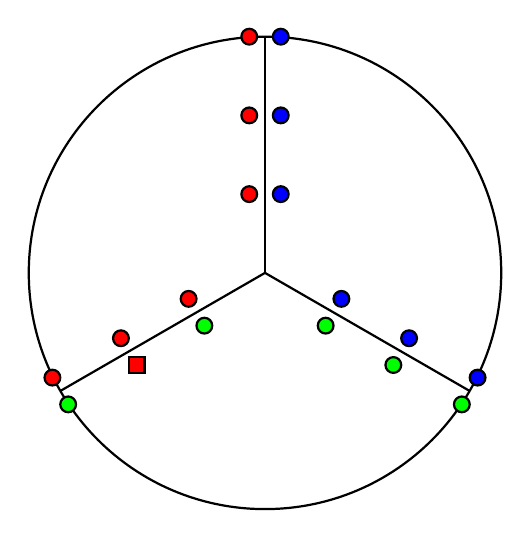
\begin{tikzpicture} [scale = 1] 
\draw[thick] (0.0, 0.0) circle [radius = 3.0];
\draw[thick] (0.0, 0.0) -- (0.0, 3.0);
\draw[fill = blue, thick] (0.2, 1.0) circle [radius = 0.1];
\draw[fill = blue, thick] (0.2, 2.0) circle [radius = 0.1];
\draw[fill = blue, thick] (0.2, 3.0) circle [radius = 0.1];
\draw[fill = red, thick] (-0.2, 1.0) circle [radius = 0.1];
\draw[fill = red, thick] (-0.2, 2.0) circle [radius = 0.1];
\draw[fill = red, thick] (-0.2, 3.0) circle [radius = 0.1];
\draw[thick] (0.0, 0.0) -- (2.6, -1.5);
\draw[fill = blue, thick] (0.97, -0.33) circle [radius = 0.1];
\draw[fill = blue, thick] (1.83, -0.83) circle [radius = 0.1];
\draw[fill = blue, thick] (2.7, -1.33) circle [radius = 0.1];
\draw[fill = green, thick] (0.77, -0.67) circle [radius = 0.1];
\draw[fill = green, thick] (1.63, -1.17) circle [radius = 0.1];
\draw[fill = green, thick] (2.5, -1.67) circle [radius = 0.1];
\draw[thick] (0.0, 0.0) -- (-2.6, -1.5);
\draw[fill = red, thick] (-0.97, -0.33) circle [radius = 0.1];
\draw[fill = red, thick] (-1.83, -0.83) circle [radius = 0.1];
\draw[fill = red, thick] (-2.7, -1.33) circle [radius = 0.1];
\draw[fill = green, thick] (-0.77, -0.67) circle [radius = 0.1];
\draw[fill = red, thick] (-1.73, -1.27) rectangle (-1.53, -1.07);
\draw[fill = green, thick] (-2.5, -1.67) circle [radius = 0.1];
\end{tikzpicture} \captionof{figure}{Incentive Incompatible Example}\label{fig:ice}
\end{figure}
The $18$ points are located inside a unit circle, and each point is $0.004$ away from the three line segments through the origin that forms angles of $120$ degrees between them. There is one point, labeled by a square in the plot, that is on the "incorrect" side of the boundary. Suppose the point corresponds to the feature vector of an agent $i $ with private label "red", then truthfully reporting her label will lead to a multi-class logistic regression model that classifies her point as "green". The probability that this model classifies her point as "red" is $0.3290$. However, if the agent misreports her label as "blue", the resulting model classifies her point as "red" with probability $0.4966$. Therefore, by lying about her label, the agent can make the principal learn an incorrect model that classifies her point correctly and with a higher probability.
\newline \newline
However, this dataset is incentive compatible if zero-one loss is minimized when estimating the logistic parameters, and if the Bayes classifier is used with maximum likelihood estimation. In general, misreporting will always lead to a lower classification probability of the agent's true label for these classifiers.
\newline \newline
Previous work on mechanism design for machine learning with strategic data sources focus on designing robust algorithms to incentivize the data providers to report their private data truthfully. Their models mainly differ in the objective and the possible actions of the data providers (agents) and the machine learner (principal).
\newline \newline
The first group of papers focuses on principal-agent problems in which each agent's private data point is the agent's type that the agent cannot change. The only action the agents can take is whether to report their private information truthfully.
\begin{enumerate}
\item Some models assume the agents' feature vectors are public, but their labels are private. \citet*{perote2004strategy}, \citet*{chen2018strategyproof}, and \citet*{gast2013linear} focus on strategy-proof linear regression algorithms and introduced clockwise repeated median estimators, generalized resistant hyperplane estimators, and modified generalized linear squares estimators. \citet*{dekel2010incentive} investigates the general regression problem with empirical risk minimization and absolute value loss. All the previously mentioned papers assume the labels are continuous variables (regression problems), and \citet*{meir2012algorithms} assumes the labels are discrete variables (classification problems) and proposes a class of random dictator mechanisms.
\item Some models assume the agents' feature vectors are also private. \citet*{chen2019grinding} investigates such problems for linear regressions.
\item Other models do not distinguish between feature vectors and labels. Each agent has a private valuation. These problems are usually modeled as facility locations problems and the solution involves some variant of the Vickrey-Clarke-Groves or Meyerson auction. These include \citet*{dutting2017optimal}, \citet*{golowich2018deep}, \citet*{epasto2018incentive}, and \citet*{procaccia2009approximate}.
\end{enumerate}


The second group papers focus on moral-hazard problems in which each agent does not have a type but they can choose an action (with a cost) that affects the probability of obtaining the correct label. \citet*{richardsonprivately} focuses on the linear regression problem in this scenario, and \citet*{cai2015optimum} and \citet*{shah2016double} investigates the problem for more general machine learning problems. \citet*{mihailescu2010strategy} also discusses a similar problem for general machine learning algorithms.
\newline \newline
The last group of papers uses machine learning or robust statistics techniques without game-theoretic models. This group of papers include \citet*{dekel2009vox}, \citet*{dekel2009good}.
\newline \newline



\section{Logistic Regression} 

\subsection{Model and Example}
In this section, we assume the principal is training a multi-class logistic (softmax) regression. There are $n $ strategic agents each providing the label of one data point to the principal. An agent, $i $, with public feature vector, $x_{i} \in \mathbb{R}^{m}$, and private discrete label, $y_{i} \in \left\{1, 2, ..., k \right\}$, has the objective of maximizing the probability that her data point is labeled correctly by the principal's model, parameterized by the $m  \times \left(k  + 1\right)$ weights (and bias) matrix $w $. The agent can choose to report $y^{\dagger}_{i}$ to achieve the objective, with possibly $y^{\dagger}_{i} \neq  y_{i}$. Denoting the weights of the model resulting from the false report from agent $i $ by $w^\star \left(y^{\dagger}_{i}\right)$, the agent's objective can be written as,
\begin{align*}
&  \displaystyle\max_{y^{\dagger} \in \left\{1, 2, ..., k \right\}} \mathbb{P}\left\{Y = y_{i} | w^\star \left(y^{\dagger}_{i}\right), x_{i}\right\},
\end{align*}
where,
\begin{align*}
&  \mathbb{P}\left\{Y = c | w, x_{i}\right\} = \dfrac{e^{z_{i,c}}}{\displaystyle\sum_{c'=1}^{k} e^{z_{i,c'}}},
\\ &  z_{i,c} = \displaystyle\sum_{j=1}^{m} w_{j,c} x_{i,j} + b_{c} , \text{\;for\;} c \in \left\{1, 2, ..., k\right\}.
\end{align*}
The principal is not strategic and he maximizes the likelihood of the data,
\begin{align*}
&\displaystyle\max_{w} \displaystyle\sum_{i=1}^{n} \log\left(\mathbb{P}\left\{Y = y^{\dagger}_{i} | w, x_{i}\right\}\right).
\end{align*}
We consider the case without a coalition of a group of agents, so only one agent is misreporting at a time, and use the following notations,
\begin{align*}
w^\star  &= \arg\displaystyle\max_{w} \displaystyle\sum_{i=1}^{n} \log\left(\mathbb{P}\left\{Y = y_{i} | w, x_{i}\right\}\right)
\\ w^\star \left(y^{\dagger}_{i}\right) &= \arg\displaystyle\max_{w} \log\left(\mathbb{P}\left\{Y = y^{\dagger}_{i} | w, x_{i}\right) + \displaystyle\sum_{i' = 0, i' \neq  i}^{n} \log\left(\mathbb{P}\left\{Y = y_{i'} | w, x_{i'}\right\}\right),\right.
\end{align*}
\begin{df} \label{df:ic} 
A dataset is incentive incompatible with respect to a learner if there exists at least one agent $i $, and some $y^{\dagger}_{i} \neq  y_{i}$ such that,
\begin{align*}
\mathbb{P}\left\{Y = y_{i} | w^\star , x_{i}\right\} &< \mathbb{P}\left\{Y = y_{i} | w^\star \left(y^{\dagger}_{i}\right), x_{i}\right\}.
\end{align*}
A learner (algorithm) is incentive compatible if there does not exist a dataset that is incentive incompatible.
\newline \newline\end{df}
\begin{prop} \label{prop:logit} 
Multi-class logistic regression is not incentive compatible.
\end{prop}
\begin{proof} \label{proof:logitpf} 
The example described in Figure \ref{fig:ice} is a dataset that is incentive incompatible.
\\* In this example, agent $i $ reports $x_{i} \in \mathbb{R}^{2}$ and $y_{i}$ is one of $1$ (red), $2$ (green), or $3$ (blue). Suppose the red square point correspond to agent $1$ with $x_{1} = \left(-1.63, -1.17\right)$ and $y_{1} = 1$.
\begin{align*}
\mathbb{P}\left\{Y = 1 | w^\star , x_{1}\right\} &= 0.3290,
\\ \mathbb{P}\left\{Y = 1 | w^\star \left(y^{\dagger}_{1} = 3\right), x_{1}\right\} &= 0.4966.
\end{align*}
Here, parameter estimation is done using maximum likelihood estimation with BFGS, and $w^\star $ is given by, with class $1$ weights normalized to $0$,

\begin{center} \begin{tabular}{|c|c|c|c|c|}
\hline
 Class &(Intercept) &x1 &x2\\ \hline
$2$ &-$0.6053178$ &$104.9925$ &-$181.3391914$\\ \hline
$3$ &-$0.2852057$ &$209.4190$ &$0.3656777$\\ \hline
\end{tabular} \end{center}
and $w^\star \left(y^{\dagger}_{1} = 3\right)$ is given by,

\begin{center} \begin{tabular}{|c|c|c|c|c|}
\hline
 Class &(Intercept) &x1 &x2\\ \hline
$2$ &-$0.1915645$ &$3.473426$ &-$5.507418$\\ \hline
$3$ &$0.8273350$ &$4.309293$ &-$1.200060$\\ \hline
\end{tabular} \end{center}


\subsection{Zero-One Loss Logistic Regression}
It is, however, possible to change the loss function so that logistic regression is incentive compatible. Changing the loss function to absolute value $L^{1}$ loss is one possibility, due to \citet*{dekel2010incentive}. Their result on incentive compatibility of empirical risk minimization in the regression setting is applicable in our model. In addition to absolute value loss, which is not a meaningful loss function for multi-class logistic regression, zero-one loss logistic regression with deterministic predictions is also incentive compatible.
\newline \newline\end{proof}
\begin{prop} \label{prop:zolog} 
Multi-class deterministic classifiers estimated by empirical risk minimization with zero-one loss is incentive compatible.
\end{prop}
\begin{proof} \label{proof:zologpf} 
For any dataset $\left\{\left(x_{i}, y_{i}\right)\right\}_{i=1}^{n}$, and the hypothesis class $\mathcal{H}$, let the optimal classifier be,
\begin{align*}
h^\star  &= \arg\displaystyle\min_{h \in \mathcal{H}} \displaystyle\sum_{i'=1}^{n} \mathbbm{1}_{\left\{y_{i'} \neq  h\left(x_{i'}\right)\right\}}.
\end{align*}
Fix an agent $i $, her feature vector $x_{i}$, and fix other agents' reports, $\left(x_{-i}, y_{-i}\right)$, define the loss function given the classifier $h $ and report of agent $i , y^{\dagger}_{i}$ as,
\begin{align*}
\mathcal{L}\left(h, y^{\dagger}_{i}\right) &= \displaystyle\sum_{i' \neq  i} \mathbbm{1}_{\left\{y_{i'} \neq  h\left(x_{i'}\right)\right\}} + \mathbbm{1}_{\left\{y^{\dagger}_{i} \neq  h\left(x_{i}\right)\right\}}.
\end{align*}
If $y_{i} = h^\star \left(x_{i}\right)$, then the classifier is already classifying $x_{i}$ correctly, misreporting will not improve the outcome for $i $. Now let the prediction be $h^\star \left(x_{i}\right) = y^\star  \neq  y_{i}$, and suppose $h^\star $ is making $k $ mistakes, meaning,
\begin{align*}
k  &= \displaystyle\min_{h \in \mathcal{H}} \mathcal{L}\left(h^\star , y_{i}\right).
\end{align*}
Agent $i $ can misreport in the following two ways:
\end{proof}
\begin{enumerate}
\item If agent $i $ reports $y^{\dagger}_{i} = y^\star $, let the new classifier be $h^{\dagger}$, note that we must have,
\begin{align*}
\mathcal{L}\left(h^{\dagger}, y^\star \right) &\leq  k - 1,
\end{align*}
because $\mathcal{L}\left(h^{\dagger}, y^\star \right) > k - 1 = \mathcal{L}\left(h^\star , y^\star \right)$ contradicts the optimality of $h^{\dagger.}$
\\* Now suppose that agent $i $ could get her true label with $h^{\dagger}$, meaning $h^{\dagger}\left(x_{i}\right) = y_{i}$, then,
\begin{align*}
\mathcal{L}\left(h^{\dagger}, y_{i}\right) &= \mathcal{L}\left(h^{\dagger}, y^\star \right) - 1
\\ &\leq  k - 2
\\ &< \mathcal{L}\left(h^\star , y_{i}\right),
\end{align*}
which contradicts the optimality of $h^\star $. Therefore, agent $i $ cannot improve the outcome by misreporting $y^\star $.
\item If agent $i $ reports $y^{\dagger}_{i} = y' \neq  y^\star $, let the new classifier be $h^{\dagger}$, note that we must have,
\begin{align*}
\mathcal{L}\left(h^{\dagger}, y'\right) &\leq  k,
\end{align*}
because if $\mathcal{L}\left(h^{\dagger}, y'\right) > k = \mathcal{L}\left(h^\star , y'\right)$ contradicts the optimality of $h^{\dagger.}$
\\* Now suppose that agent $i $ could get her true label with $h^{\dagger}$, then,
\begin{align*}
\mathcal{L}\left(h^{\dagger}, y_{i}\right) &= \mathcal{L}\left(h^{\dagger}, y_{i}\right) - 1
\\ &\leq  k - 1
\\ &< \mathcal{L}\left(h^\star , y_{i}\right),
\end{align*}
which contradicts the optimality of $h^\star $. Therefore, agent $i $ cannot improve the outcome by misreporting $y'$.
\\* Therefore, no agent can improve the outcome and the dataset is incentive compatible.
\newline \newline
\end{enumerate}




\section{Bayes Classifier} 
The example given previously is incentive compatible with respect to the Naive Bayes classifier. None of the agents have the incentive to misreport their labels. This is always true in general for any parametric Bayesian classifier estimated using maximum likelihood.
\newline \newline
\begin{prop} \label{prop:bc} 
Bayesian classifiers are incentive compatible.
\end{prop}
\begin{proof} \label{proof:bcpf} 
Suppose the loglikelihood function of class $y $ given the feature vector $x $ and the parameter $w $ is $\ell\left(x ; w \right)$, and define the optimal parameter, $w^\star $ for class $y_{i}$, of the truthful model as,
\begin{align*}
w^\star  &= \arg\displaystyle\max_{w} \displaystyle\sum_{i' : y_{i'} = y_{i}} \ell\left(x_{i'} ; w\right)
\\ &= \arg\displaystyle\max_{w} \displaystyle\sum_{i' \neq  i : y_{i'} = y_{i}} \ell\left(x_{i'} ; w\right) + \ell\left(x_{i} ; w\right).
\end{align*}
Let the optimal parameter when agent $i $ reports $y^{\dagger}_{i} \neq  y_{i}$ be $w^{\dagger,}$
\begin{align*}
w^{\dagger} &= \arg\displaystyle\max_{w} \displaystyle\sum_{i' \neq  i: y_{i'} = y_{i}} \ell\left(x_{i'} ; w\right).
\end{align*}
In particular, these implies the following optimality conditions,
\begin{align*}
\displaystyle\sum_{i' \neq  i : y_{i'} = y_{i}} \ell\left(x_{i'} ; w^\star \right) + \ell\left(x_{i} ; w^\star \right) &\geq  \displaystyle\sum_{i' \neq  i : y_{i'} = y_{i}} \ell\left(x_{i'} ; w^{\dagger}\right) + \ell\left(x_{i} ; w^{\dagger}\right),
\\ \displaystyle\sum_{i' \neq  i: y_{i'} = y_{i}} \ell\left(x_{i'} ; w^{\dagger}\right) &\geq  \displaystyle\sum_{i' \neq  i: y_{i'} = y_{i}} \ell\left(x_{i'}, w^\star \right).
\end{align*}
Taking the difference between the two inequalities, we have,
\begin{align*}
\ell\left(x_{i} ; w^\star \right) &\geq  \ell\left(x_{i} ; w^{\dagger}\right).
\end{align*}
Note that the empirical prior probability for class $y_{i}$ is decreased if the number of data with label $y_{i}$ is decreased by $1$. Therefore, the posterior probabilities satisfy,
\begin{align*}
\mathbb{P}\left\{y_{i} | x_{i}, w^\star \right\} &\geq  \mathbb{P}\left\{y_{i} | x_{i}, w^{\dagger}\right\}.
\end{align*}
Therefore, no agent can improve the outcome and the dataset is incentive compatible.
\newline \newline\end{proof}
\bibliographystyle{te}
\bibliography{cs}


\end{document}
